%  !TeX  root  =  user_guide.tex

\section{Модуль Преобразователь Dxf2Shp}\label{dxf2shape}

% когда переработка раздела будет завершена,
% раскоментируйте следующую строку:
% \updatedisclaimer

Модуль <<Преобразователь Dxf2Shp>> может быть использован для преобразования
векторных данных из формата DXF в формат shape-файлов. Перед его
использованием должны быть определены следующие параметры:

\begin{itemize}
\item \textbf{Входной DXF-файл}: Введите путь к файлу в формате DXF,
который необходимо преобразовать
\item \textbf{Выходной shp-файл}: Введите любое желаемое имя файла для
создаваемого shape-файла
\item \textbf{Тип выходного файла}: Определите тип геометрии данных
выходного shape-файла. В настоящее время поддерживаются такие типы как
полилиния, полигон и точка.
\item \textbf{Экспорт текстовых меток}: При выборе данного пункта
дополнительно будет создан shape-файл слоя точек с
таблицей DBF, которая содержит информацию о полях <<TEXT>>, найденных в
файле DXF и соответствующие текстовые строки.
\end{itemize}

\begin{figure}[ht]
   \centering
   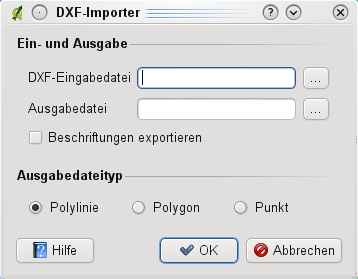
\includegraphics[clip=true, width=12cm]{dxf2shape_dialog}
   \caption{Модуль <<Преобразователь Dxf2Shp>> \wincaption}\label{fig:dxf2shape_dialog}
\end{figure}

\minisec{Использование модуля}

\begin{enumerate}
  \item Запустите QGIS, загрузите модуль Dxf2Shp в Менеджере модулей
  (см. Раздел~\ref{sec:load_core_plugin}) и нажмите кнопку
  \toolbtntwo{dxf2shp_converter}{Dxf2Shp Converter}, расположенную на
  панели инструментов QGIS. Диалоговое окно модуль Dxf2Shp показано на
  Рисунке~\ref{fig:dxf2shape_dialog}.
  \item Введите имя входного DXF файла, укажите имя выходного shape-файла
  и его тип.
  \item Выберите пункт \checkbox{Экспорт текстовых меток}, если вам
  требуется создать дополнительный слой, содержащий надписи.
  \item Нажмите кнопку \button{Ok}.
\end{enumerate}

\FloatBarrier
